\exercise{Degree correlations}{4}
Let us once again consider a network where 75\% of the nodes have degree 1 and 25\% degree 3. 

\subquestion 
Determine if a giant component exists, and if so, compute it's size.

\solution
We follow the usual procedure. The degree distribution is 
\eq{
p_k = \frac{3}{4}\delta_{k,1}+\frac{1}{4}\delta_{k,3}.
}
Therefore the mean degre is 
\eq{
z=\sum kp_k = 1.5,
}
and the excess degree distribution is 
\eq{
q_k=\frac{(k+1)p_{k+1}}{z} = \frac{\delta_{k,0}+\delta_{k,2}}{2}.
}
Therfore,
\eq{
q=\sum k q_k = 1
}
SO we are just at the point where the giant component is forming. We can argue that it technically exists already but it's size is still 
$s=0$.

\subquestion
So far we have considered the case where the nodes are connected completely randomly, but what if the network is not quite so random? Perhaps the nodes of degree 3 like to link to their own kind? Use $p_{i,j}$ to denote the probability that a link starting at a node of degree $i$ leads to a node of degree $j$. Suppose we know $p_{3,3}=b$, and compute $p_{3,1}$, $p_{1,3}$ and $p_{1,1}$.

\solution
Because a link starting at a node of degree three will lead to a node of degree with probability $b$, it must lead to a node of degree 1 with probability 
\eq{
p_{3,1}=1-b
}
The other two are more tricky, but as always we can make it a bit easier by thinking in terms of endpoints. In a network of size $N$ there are $3N/4$ nodes of degree 1, so the total number of endpoints of nodes of degree 1 is also $3N/4$. 

We also know that there are $N/4$ nodes of degree 3. Each of them has three links of which a proportion $1-b$ lead to nodes of degree 1. Hence the number of endpoints on nodes of degree 1 at which a link to a node of degree 3 starts is $(1-b)3N/4$. Therefore the probability that a link from a node of degree 1 leads to a node of degree 3 is 
\eq{
p_{13}=\frac{(1-b)3N/4}{3N/4} = 1-b
}
Just like $p_{3,3}$ and $p_{3,1}$, the two numbers $p_{1,3}$ and $p_{1,1}$ must add up to 1. Hence 
\eq{
p_{1,1}=1-(1-b)=b,
}
nice!

\subquestion 
Find a way to compute the giant component size as a function of $b$. In your calculation use $s_i$ to denote the probability that a node of degree $i$ is part of the giant component. Use your result to compute the giant component size for $b=3/4$.

\solution
 Let's start by thinking of nodes of degree 1. We know that with probability $p_{1,1}=b$ the node's single link leads to another node of degree 1. In this case the node is certainly not part of the giant component. Conversely, with probability $p_{1,3}$ the node's single link leads to a node of degree 3 and then the degree-1 node is part of the giant component if the degree-3 node is also part of the giant component. 
 
 Let us use $w$ to denote the probability that a node of degree 3 that we have reached via a link is not part of the giant component. In other words, a link to a degree-3 node connects us to the giant component with probability $1-w$. Hence we can write,
 \eq{
 s_1=p_{1,3}(1-w)=(1-b)(1-w)
 }
 This was a good warm up. Let's tackle $s_3$, we can almost try our usual approach
 \eq{
 s_3=1-v^3,
 }
 which is saying a node of degree us part of the giant component (probability 1), unless none of it's three links connect it to the giant component (probability $v^3$). So, $v$ in this case is the probability that a link from degree-3 node does not connect us to the giant component. To link $v$ and $w$ consider that a link from a degree-3 node leads to a node of degree 1 with probability $p_{3,1}$. In this case it does not connect us to the giant component with probability 1. Conversely, a link from a degree-3 node leads to another degree-3 node with probability $p_{3,3,}$ and in this case it does not connect us to the giant component with probability $w$. Hence,
 \eq{
 v=p_{3,1}1 + p_{3,3}w = 1-b + b w = 1-b(1-w)
 }
 Now we only need to compute $w$ and everything will unravel. So we need to consider a node of degree 3 that we have reached via a link. This node does not connect us to the giant component if none of it's other two link connect to the giant component, hence
 \eq{
 w=v^2 
 }
 substituting into the equation above we can now solve
 \eqa{
 v&=&1-b(1-v^2) \\
 0&=&bv^2-v-b+1 \\
 0&=&bv-1-b \\
 v&=&(1-b)/b
 }
 where we divided out the known solution $v=1$ in the third step by dividing by $v-1$.
 
 This calculation is a tough nut, so let's build some confidence by considering some limiting cases. If we set $b=1$ then all links from nodes of degree 3 lead to other nodes of degree 3. Since the nodes of degree three no longer interact with nodes of degree one, they start behaving like a homogeneous network of degree 3 and we know that in such a network all nodes are in the giant component, hence it is no surprise that $v=0$ in this limit. if we set $b=1/2$ then we are back to the case of completely random connections, that we studied in part a. In this case we get $v=1$ which isn't surprising since we know that the giant has size $s=0$ in this case, so it is consistent that links do not connect us to the giant component with probability 1. If we chose $b<1/2$ we get values of $v>1$ which can't be interpreted as probabilities. This happens because we are now considering a case where the giant component no longer exists so trying to compute it's size yields erroneous results.     
 
  It is useful to define 
 \eq{
 \bar{b}=1-b
 }
 such that 
 \eq{
 v=\frac{\bar{b}}{b}
 }
 We can now write 
 \eq{
 w=v^2=\frac{\bar{b}^2}{b^2}
 }
 which allows us to write 
 \eq{
 s_1=(1-b)(1-w)=(1-b)(1-\bar{b}^2/b^2)= \bar{b}-\frac{\bar{b}^3}{b^2} 
 }
 \eq{
 s_3=1-v^3=1-\frac{\bar{b}^3}{b^3} 
 }
 and hence 
 \eqa{
 s&=&\frac{3}{4}s_1 + \frac{1}{4}s_3 \\
  &=&\frac{3}{4}*\left(\bar{b}-\frac{\bar{b}^3}{b^2}\right)+\frac{1}{4}\left(1-\frac{\bar{b}^3}{b^3}\right). 
 }
 If we substitute in $b=3/4$ we find 
 \eq{s=\frac{11}{27}.}
 For $b=3/4$ the networks has positive degree correlations (it is assortative) because high degree nodes are more likely to link to high degree nodes than they would be in the networks where links are connect random nodes. The take home message from this calculation is that networks with such degree correlations can have larger giant components than random networks. In this case the result is particularly impressive increasing the size of the giant component from 0 to more than 40\% of the network. 
 
 As a bonus, here is a plot of the giant component size as a function of $b$
 \begin{center}
 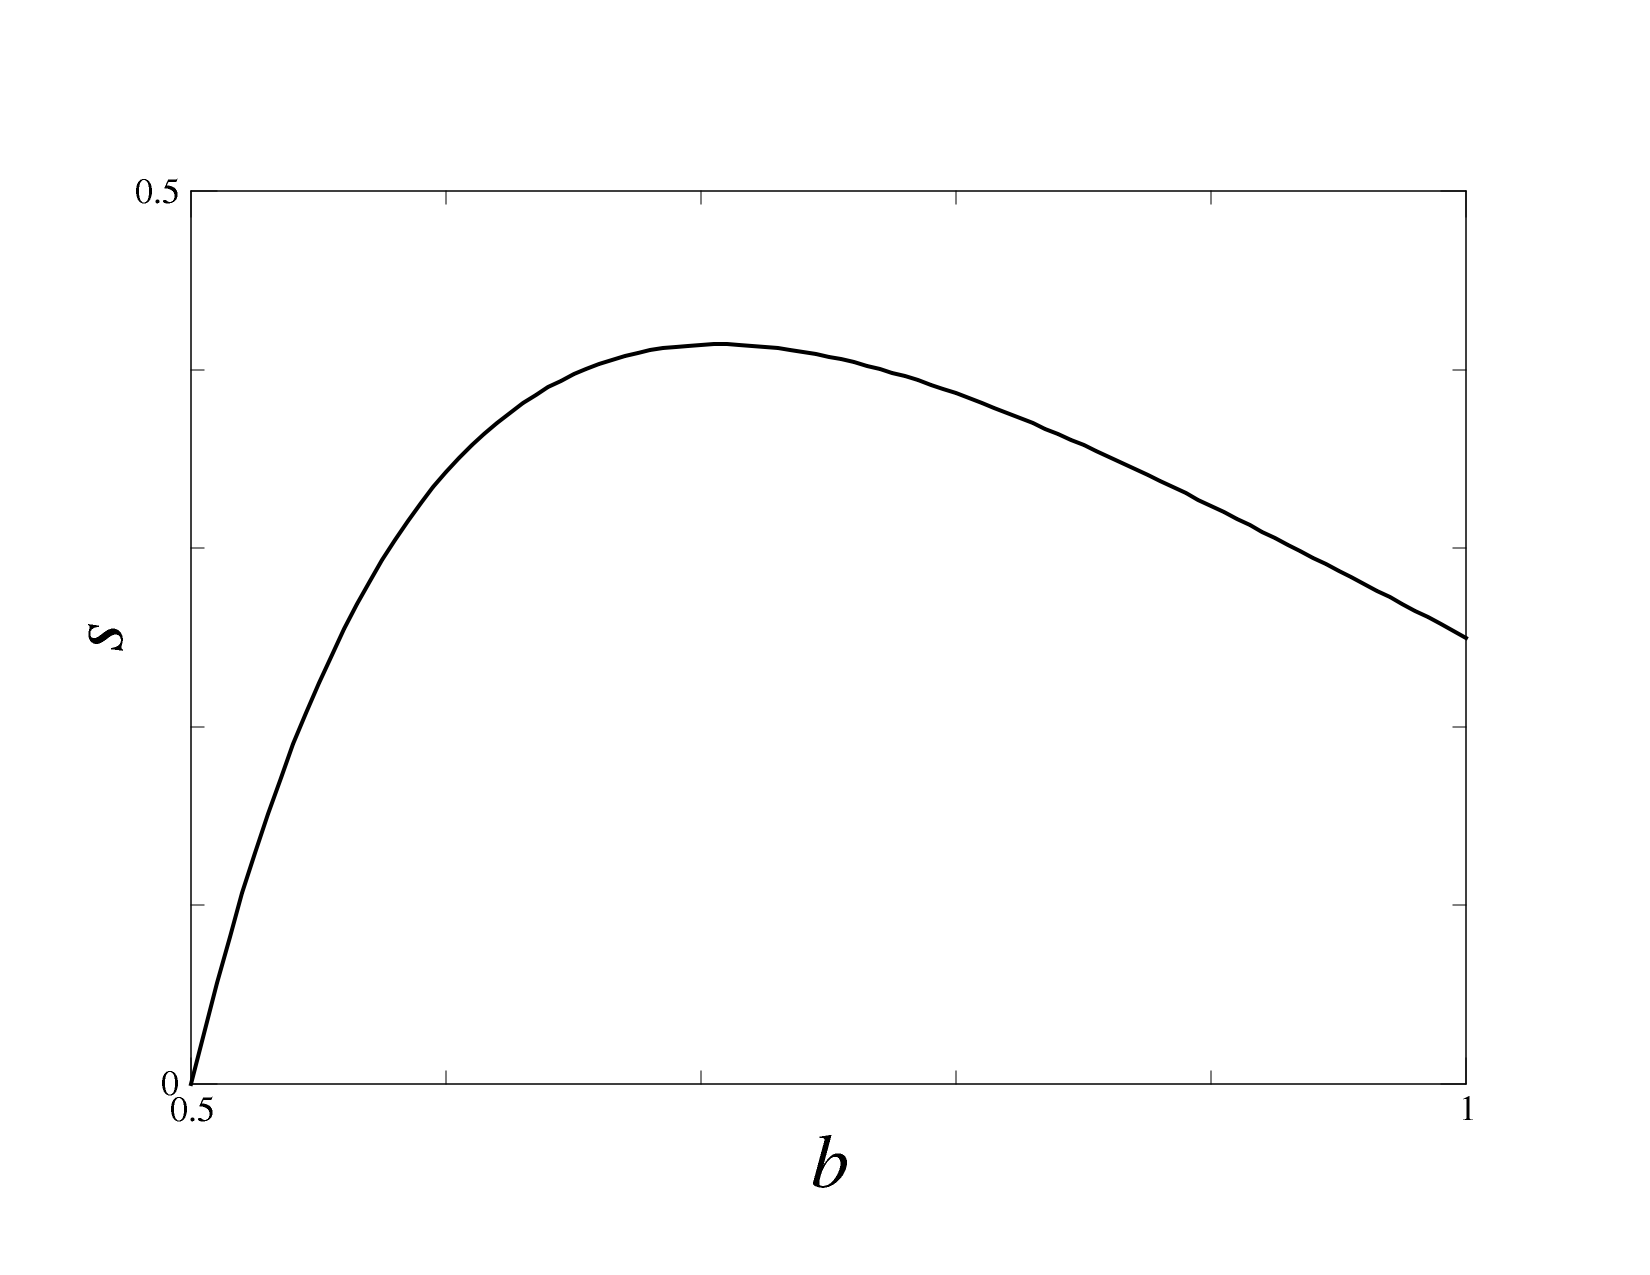
\includegraphics[width=0.6\textwidth]{assort}     
 \end{center}
\solutionend